\chapter{What Animals Eat}\label{ch:g2:what-animals-eat}

The rabbit in the meadow nibbles grass all day. The fox that
crosses the same meadow at dusk is not interested in grass at all
--- it is interested in the rabbit. And the blackbird takes worms
in the morning and cherries in the afternoon. Every \omterm{def:g1:animals-around-us:animal}{animal} must
eat, but not every \omterm{def:g1:animals-around-us:animal}{animal} eats the same things.

\section{Three kinds of eaters}

\begin{definition}[Herbivore, carnivore, omnivore]\label{def:g2:what-animals-eat:kinds}
\omterm{def:g1:animals-around-us:animal}{Animals} are sorted by what they eat:
\begin{itemize}
  \item a \emph{herbivore}\index{herbivore} eats \omterm{def:g1:plants-around-us:plant}{plants}: grass,
        \omterm{def:g1:plants-around-us:parts}{leaves}, \omterm{def:g2:from-seed-to-plant:seed}{seeds}, fruit --- the rabbit, the cow, the snail;
  \item a \emph{carnivore}\index{carnivore} eats other \omterm{def:g1:animals-around-us:animal}{animals}:
        the fox, the cat, the ladybug (which hunts tiny \omterm{def:g1:plants-around-us:plant}{plant}
        lice);
  \item an \emph{omnivore}\index{omnivore} eats both \omterm{def:g1:plants-around-us:plant}{plants} and
        \omterm{def:g1:animals-around-us:animal}{animals}: the blackbird, the wild boar --- and humans.
\end{itemize}
\end{definition}

\begin{example}[One meadow, three menus]\label{ex:g2:what-animals-eat:meadow}
In one summer meadow: the rabbit crops the grass (\omterm{def:g2:what-animals-eat:kinds}{herbivore}); the
fox hunts the rabbit (\omterm{def:g2:what-animals-eat:kinds}{carnivore}); the blackbird takes a worm now,
a cherry later (\omterm{def:g2:what-animals-eat:kinds}{omnivore}). Three neighbors, three menus --- and
notice that the fox's dinner ate grass first.
\end{example}

\begin{omfigure}
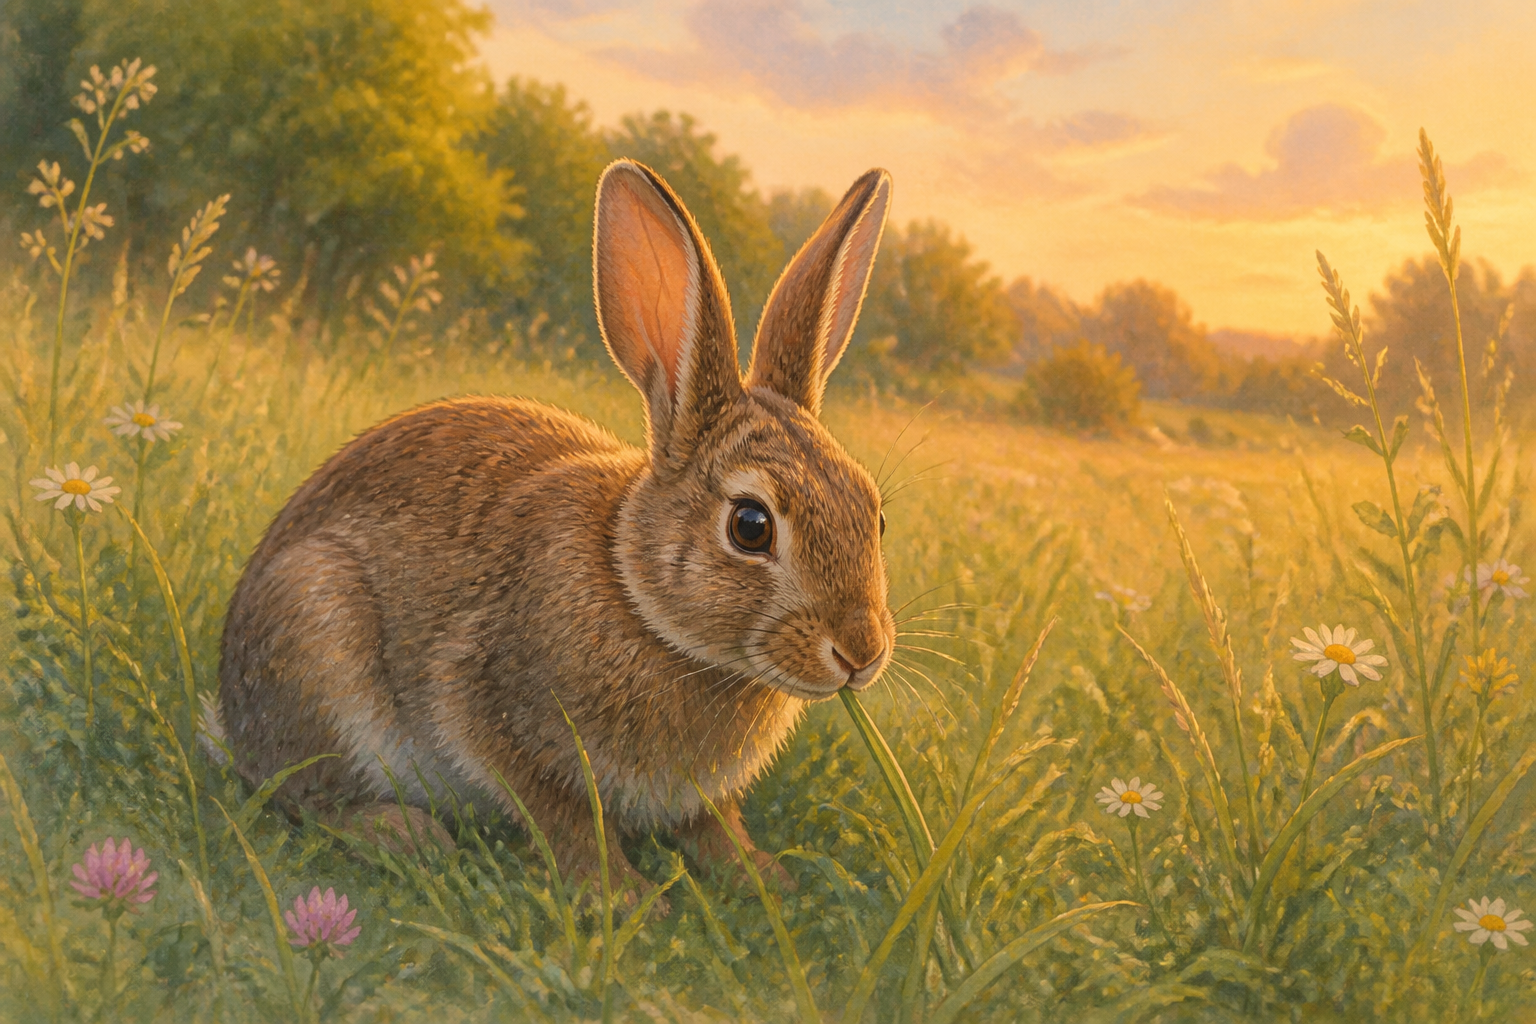
\includegraphics[width=0.6\linewidth]{images/book1/ai/g2-eat-rabbit.png}

{\small A \omterm{def:g2:what-animals-eat:kinds}{herbivore} at work: the rabbit and the meadow, blade by
blade.}
\end{omfigure}

\begin{remark}[Carnivores are not villains]\label{rem:g2:what-animals-eat:fox}
The fox is not ``mean'' for eating rabbits: hunting is simply how
a \omterm{def:g2:what-animals-eat:kinds}{carnivore} feeds --- as natural as the rabbit's nibbling. In
nature, eating and being eaten are part of how life works; a later
chapter will hang all these meals together into food chains.
\end{remark}

\section{Reading an animal's menu from its body}

\begin{proposition}[Bodies match menus]\label{prop:g2:what-animals-eat:match}
An \omterm{def:g1:animals-around-us:animal}{animal}'s body carries clues about its food:
\begin{itemize}
  \item \omterm{def:g2:what-animals-eat:kinds}{herbivores} like the rabbit and the cow have big flat
        cheek teeth for grinding \omterm{def:g1:plants-around-us:plant}{plants}, and spend long hours
        eating;
  \item \omterm{def:g2:what-animals-eat:kinds}{carnivores} like the cat and the fox have pointed teeth for
        seizing prey, sharp claws, and forward-looking \omterm{def:g1:the-five-senses:sense}{eyes} for
        hunting;
  \item birds show it in the beak: short and thick for cracking
        \omterm{def:g2:from-seed-to-plant:seed}{seeds} (the sparrow), curved and hooked for tearing meat
        (the eagle), long and thin for picking insects from bark.
\end{itemize}
\end{proposition}
\admitted

\begin{omfigure}
\begin{minipage}[t]{0.31\linewidth}\centering
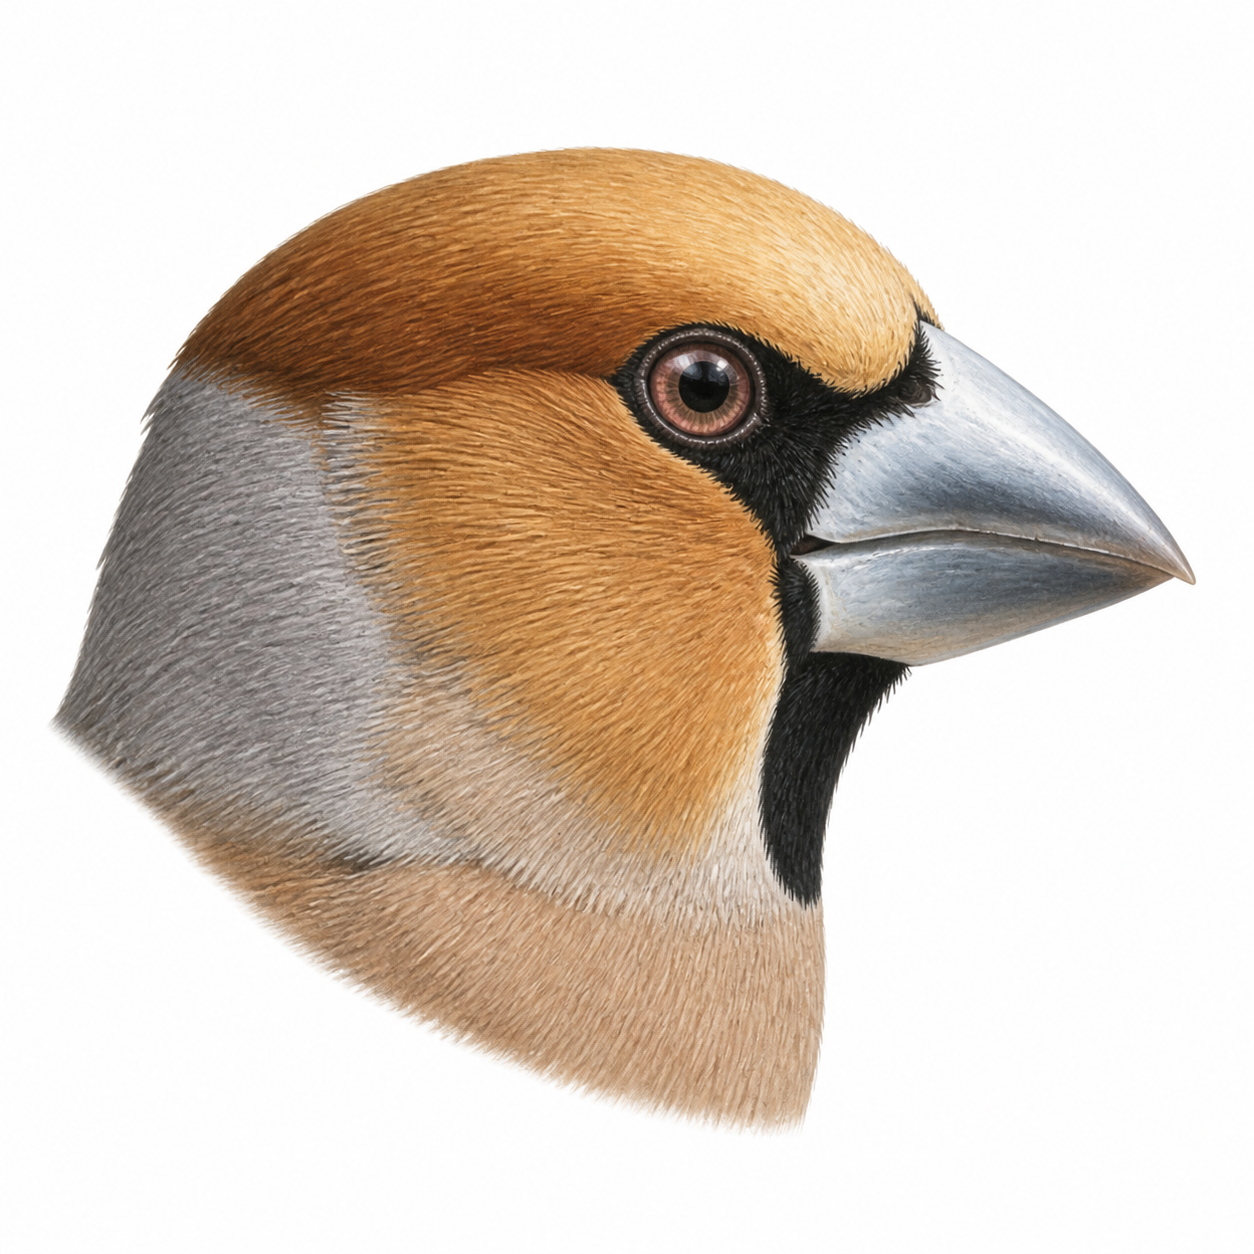
\includegraphics[width=\linewidth]{images/book1/ai/fig-beak-seed.png}

{\small short thick beak:\\ cracks \omterm{def:g2:from-seed-to-plant:seed}{seeds}}
\end{minipage}\hfill
\begin{minipage}[t]{0.31\linewidth}\centering
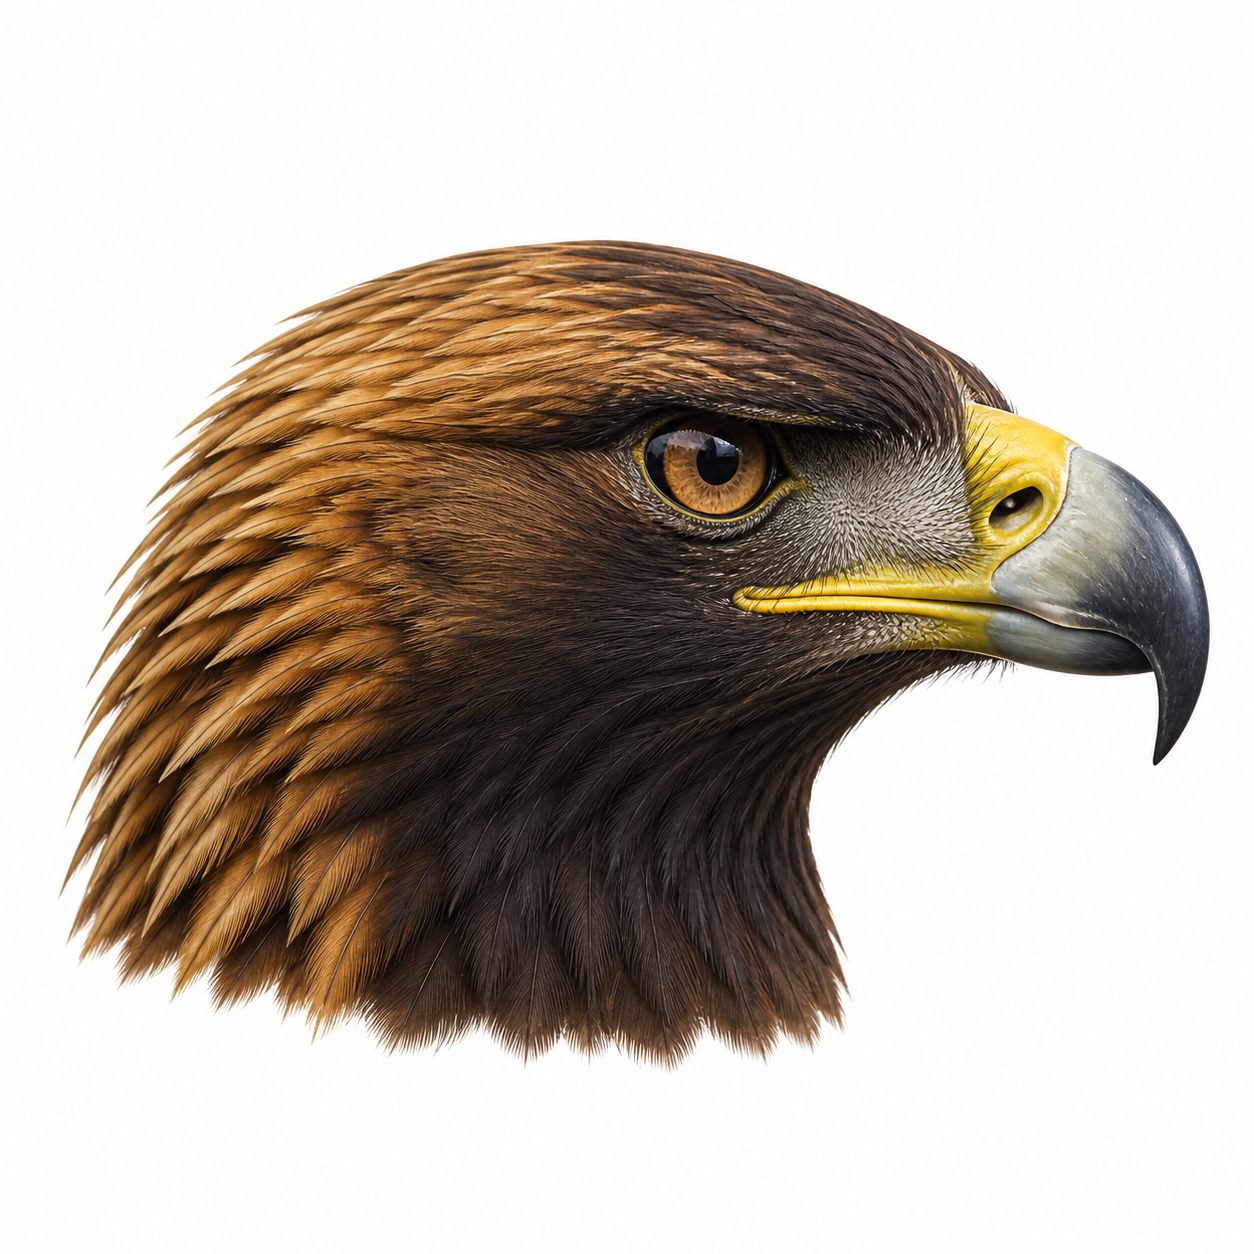
\includegraphics[width=\linewidth]{images/book1/ai/fig-beak-hook.png}

{\small hooked beak:\\ tears meat}
\end{minipage}\hfill
\begin{minipage}[t]{0.31\linewidth}\centering
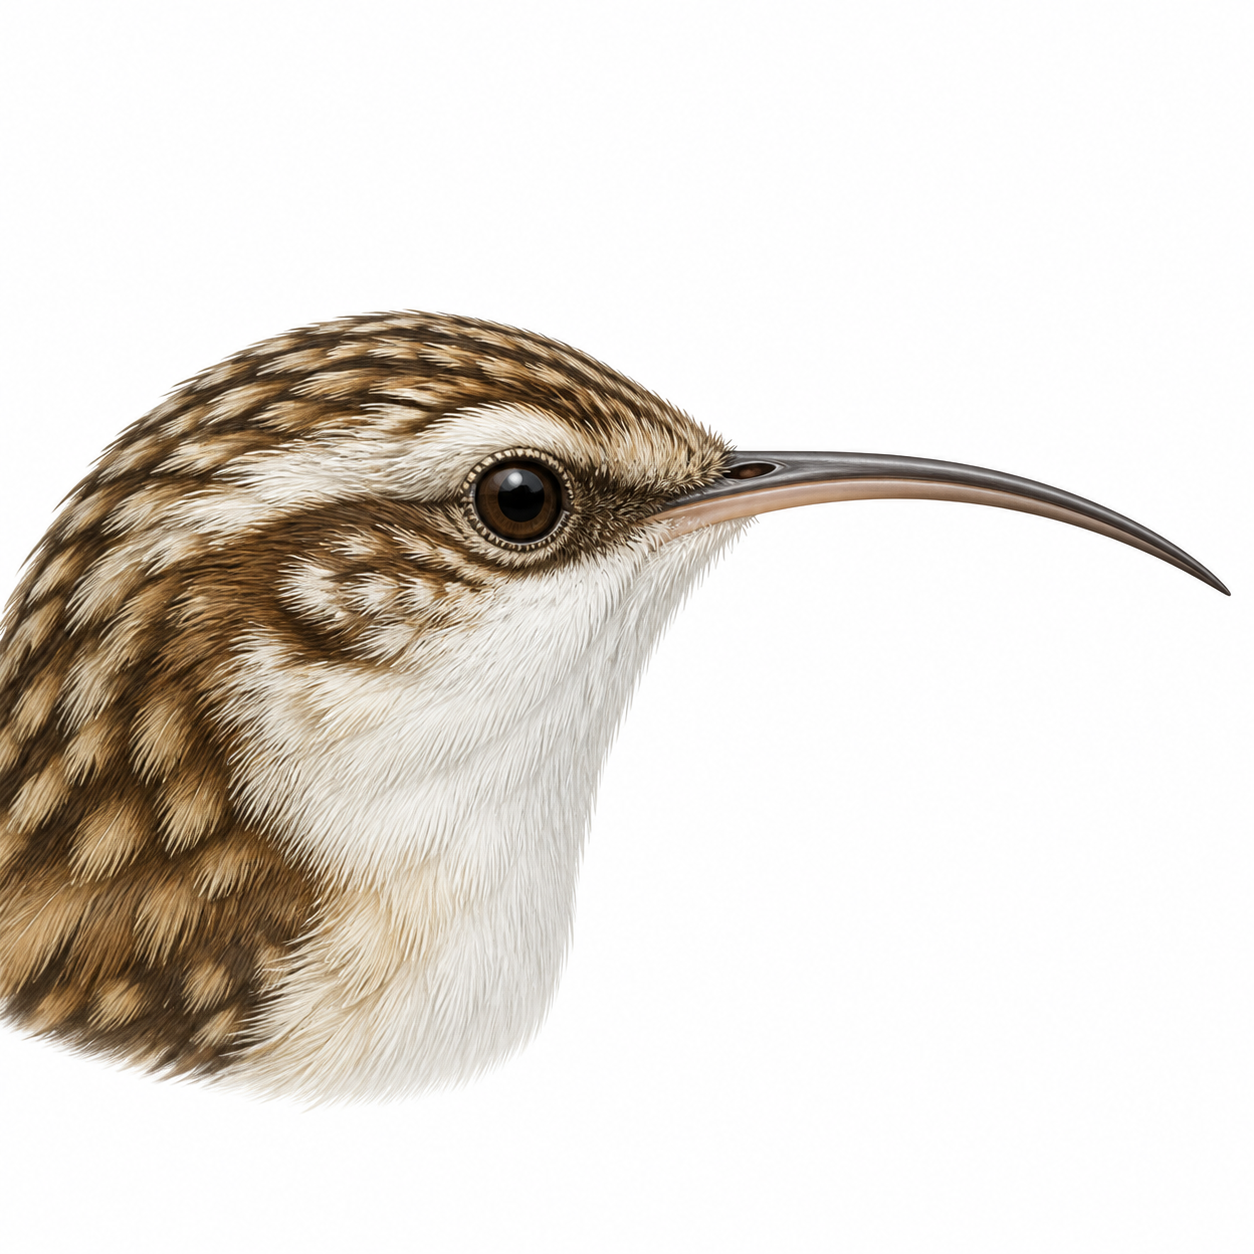
\includegraphics[width=\linewidth]{images/book1/ai/fig-beak-thin.png}

{\small long thin beak:\\ picks out insects}
\end{minipage}

\medskip
{\small Three beaks, three menus: the bird's beak is a tool shaped
by its food.}
\end{omfigure}

\begin{example}[The cat's teeth]\label{ex:g2:what-animals-eat:cat}
Watch a cat yawn: long pointed teeth at the front corners of its
mouth. Those are seizing teeth --- a \omterm{def:g2:what-animals-eat:kinds}{carnivore}'s equipment. The
cow, yawning, would show none: her mouth is all wide, flat
grinders for grass.
\end{example}

\begin{method}[Guessing a menu]\label{met:g2:what-animals-eat:guess}
To guess what an unknown \omterm{def:g1:animals-around-us:animal}{animal} eats:
\begin{enumerate}
  \item look at the teeth or the beak: flat grinders, pointed
        seizers, or both?
  \item look at claws and \omterm{def:g1:the-five-senses:sense}{eyes}: hunting tools, or not?
  \item watch it feed if you can --- the surest clue of all;
  \item then name it: \omterm{def:g2:what-animals-eat:kinds}{herbivore}, \omterm{def:g2:what-animals-eat:kinds}{carnivore} or \omterm{def:g2:what-animals-eat:kinds}{omnivore}.
\end{enumerate}
\end{method}

\section{Eating enough, day after day}

\begin{proposition}[Feeding is a daily task]\label{prop:g2:what-animals-eat:daily}
Food is the body's fuel and building material, so \omterm{def:g1:animals-around-us:animal}{animals} must eat
again and again, day after day. How much time it takes depends on
the menu: grass gives little at each mouthful, so the cow grazes
for hours; meat is rich, so the fox may eat one good meal and rest.
\end{proposition}
\admitted

\begin{example}[Winter changes the menu]\label{ex:g2:what-animals-eat:winter}
Food changes with the seasons. The blackbird eats worms and
insects in summer, but in winter, when the ground is hard, it
switches to berries. An \omterm{def:g2:what-animals-eat:kinds}{omnivore}'s wide menu is a great help when
times get hard.
\end{example}

\section{Exercises}

\begin{exercise}[$\star$]\label{exo:g2:what-animals-eat:1}
Give the words for: an \omterm{def:g1:animals-around-us:animal}{animal} that eats \omterm{def:g1:plants-around-us:plant}{plants}; an \omterm{def:g1:animals-around-us:animal}{animal} that
eats other \omterm{def:g1:animals-around-us:animal}{animals}; an \omterm{def:g1:animals-around-us:animal}{animal} that eats both.
\end{exercise}

\begin{exercise}[$\star$]\label{exo:g2:what-animals-eat:2}
\omterm{def:g2:what-animals-eat:kinds}{Herbivore}, \omterm{def:g2:what-animals-eat:kinds}{carnivore} or \omterm{def:g2:what-animals-eat:kinds}{omnivore}: (a) the cow; (b) the fox; (c)
the blackbird; (d) the snail; (e) the human?
\end{exercise}

\begin{exercise}[$\star$]\label{exo:g2:what-animals-eat:3}
Which teeth does a \omterm{def:g2:what-animals-eat:kinds}{herbivore} need most: flat grinders, or pointed
seizers? Why?
\end{exercise}

\begin{exercise}[$\star$]\label{exo:g2:what-animals-eat:4}
Match each beak with a menu: short and thick; curved and hooked;
long and thin.
\end{exercise}

\begin{exercise}[$\star$]\label{exo:g2:what-animals-eat:5}
The ladybug is small, pretty --- and a \omterm{def:g2:what-animals-eat:kinds}{carnivore}. What does it
hunt?
\end{exercise}

\begin{exercise}[$\star$]\label{exo:g2:what-animals-eat:6}
Why does the cow spend many more hours eating than the fox does?
Use \cref{prop:g2:what-animals-eat:daily}.
\end{exercise}

\begin{exercise}[$\star$]\label{exo:g2:what-animals-eat:7}
What does the blackbird eat in summer, and in winter? Why is a
wide menu useful?
\end{exercise}

\begin{exercise}[$\star$]\label{exo:g2:what-animals-eat:8}
Try it: watch birds in a park or at a feeder. Note what each kind
takes --- \omterm{def:g2:from-seed-to-plant:seed}{seeds}, bread, insects, berries --- and look at their
beaks. Does \cref{prop:g2:what-animals-eat:match} hold?
\end{exercise}

\begin{exercise}[$\star\star$]\label{exo:g2:what-animals-eat:9}
A zoo receives a mystery \omterm{def:g1:animals-around-us:animal}{animal}: pointed front teeth, sharp
claws, \omterm{def:g1:the-five-senses:sense}{eyes} facing forward. What is its likely menu? Which steps
of \cref{met:g2:what-animals-eat:guess} did you use?
\end{exercise}

\begin{exercise}[$\star\star$]\label{exo:g2:what-animals-eat:10}
``Without grass there would soon be no foxes.'' The fox never
eats grass --- yet the sentence is right. Explain, using the
meadow of \cref{ex:g2:what-animals-eat:meadow}.
\end{exercise}
